\documentclass[main]{subfiles}

\begin{document}
	\begin{Theorem}[непрерывный образ компатка]
		\[f \in C(E, \R^m) \rla f: E \to \R^m \text{ --- непр. в } E\]
		\[K \text{ --- компакт,} \q K \subset \R^n,\q f \in C(K, \R^m)\]
		\[\text{Тогда } f(K) \text{ --- компакт}\]
	\end{Theorem}

	\begin{Proof} \
		\center{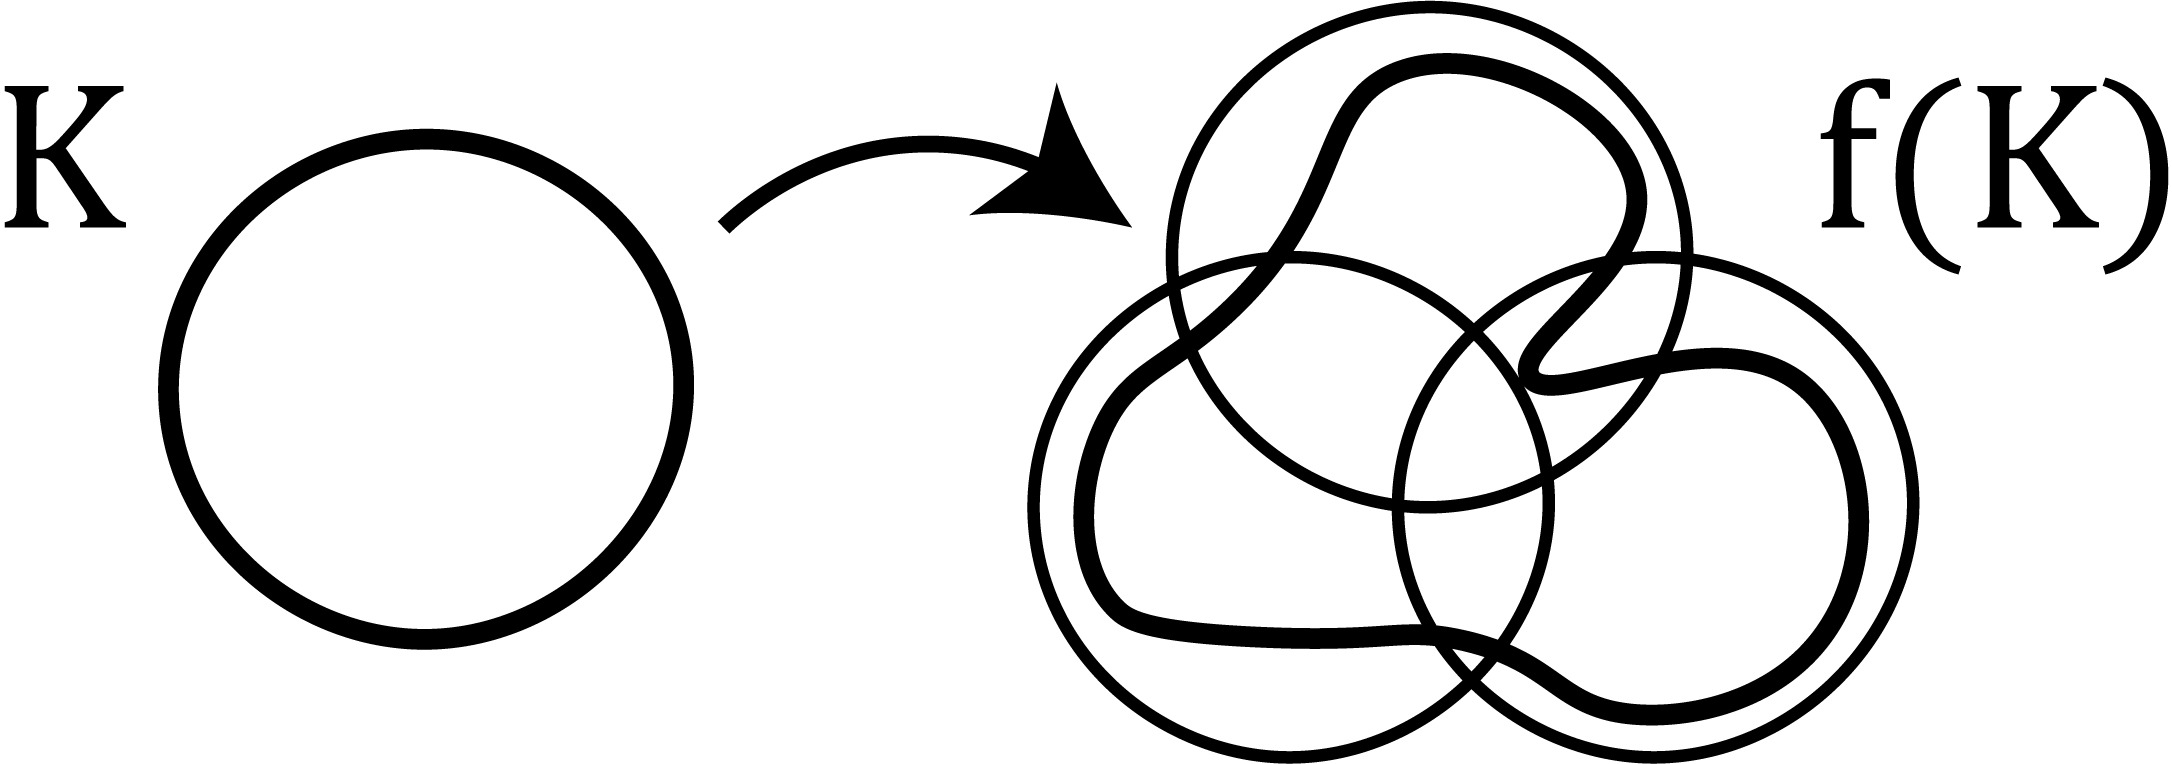
\includegraphics[width = 4cm]{pics/3_1}}
		\[\text{Пусть } \{U_\alpha\}_{\alpha \in A} \text{ --- откр. покр. } f(K)  \]
		\[f(K) \subset \bigcup_{\alpha \in A} U_\alpha \]
		\[\Ra f^{-1} (U_\alpha) \text{ - откр., причем}\]
		\[K \subset \bigcup_{\alpha \in A} f^{-1} (U_\alpha)  \text{ --- откр. покр. комп. } \RA
			\exists f^{-1} (U_\alpha_1) ... f^{-1} (U_{\alpha_N} )\]
		\[K \subset \bigcup_{k = 1}^N f^{-1} (U_{\alpha_k} ) \RA f(K) \subset \bigcup_{k = 1}^N U_{\alpha_k}\]
		\[\text{ --- выделили конечное подпокрытие} \RA f(K) \text{ --- компакт}\]
	\end{Proof}

	\newpage
	\subsection{Локальные и глобальные свойства непрерывных отображений. Доказательство теоремы Вейерштрасса}

	\begin{Theorem}[Вейерштрасса]
		\[K \text{ --- компакт; } f \in C(K, \R^m), \text{ тогда:}\]
		\begin{enumerate}
			\item $f$ --- огр.
			\item Если m = 1, то f достигает $\sup$ и $\inf$ на K
		\end{enumerate}
	\end{Theorem}

	\begin{Proof}
		\[f: K \to \R^m \text{ --- огр.} \rla \exists M : \forall x \in K \q d(f(x), 0) < M\]
		\begin{figure}[H]
			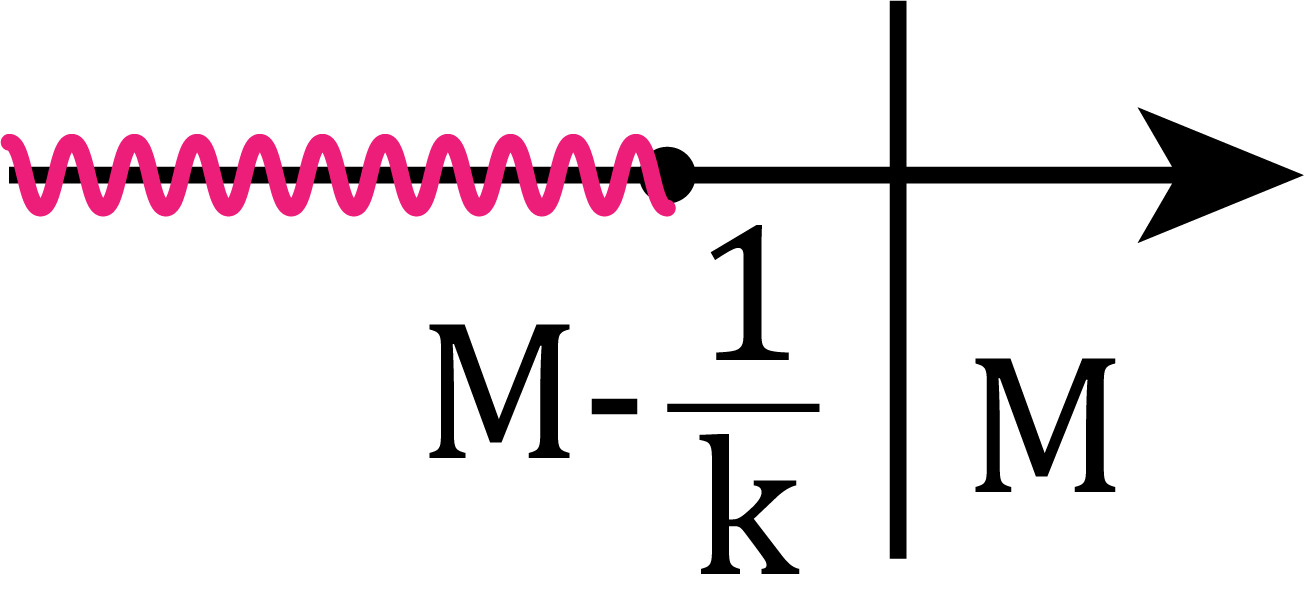
\includegraphics[width = 3cm]{pics/3_2}
			\centering
		\end{figure}
		\begin{enumerate}
			\item $f(K)$ - комп. $\Ra$ огр.
			\item $\displaystyle f : K \to \R \RA  M = \sup_{x \in K} f(x) < +\infty$
			      \[\forall k \in \N \q \exists x^k \in K:\]
			      \[M - \frac{1}{k} < f(x^k) \leq M \RA f(x^k) \underset{k \to  \infty}{\to} M\]
			      \[f(x^k) \in f(K) \text{ --- компакт } \RA \text{ замкн.}\]
			      \[\Ra \text{ сод. все свои пред. т.}\RA M \in f(K)\]
		\end{enumerate}
	\end{Proof}

	\newpage
	\subsection{Локальные и глобальные свойства непрерывных отображений. Доказательство теоремы Кантора}

	\begin{Theorem} [Кантора]
		\[f \in C(K, \R^m) \q K \subset \R^n \text{ --- компакт } \RA f \text{ --- равном. непр. на } K \]
	\end{Theorem}

	\begin{Proof}
		\[f \text{ - непр. } \Ra \text{ непр. } \forall x \in K \q \forall \mathcal{E} > 0 \q \exists \delta_x :\]
		\[\forall x' \in K \q d(x', x) < 2 \delta_x \RA d(f(x'), f(x)) < \frac{\mathcal{E}}{2}\]
		\center{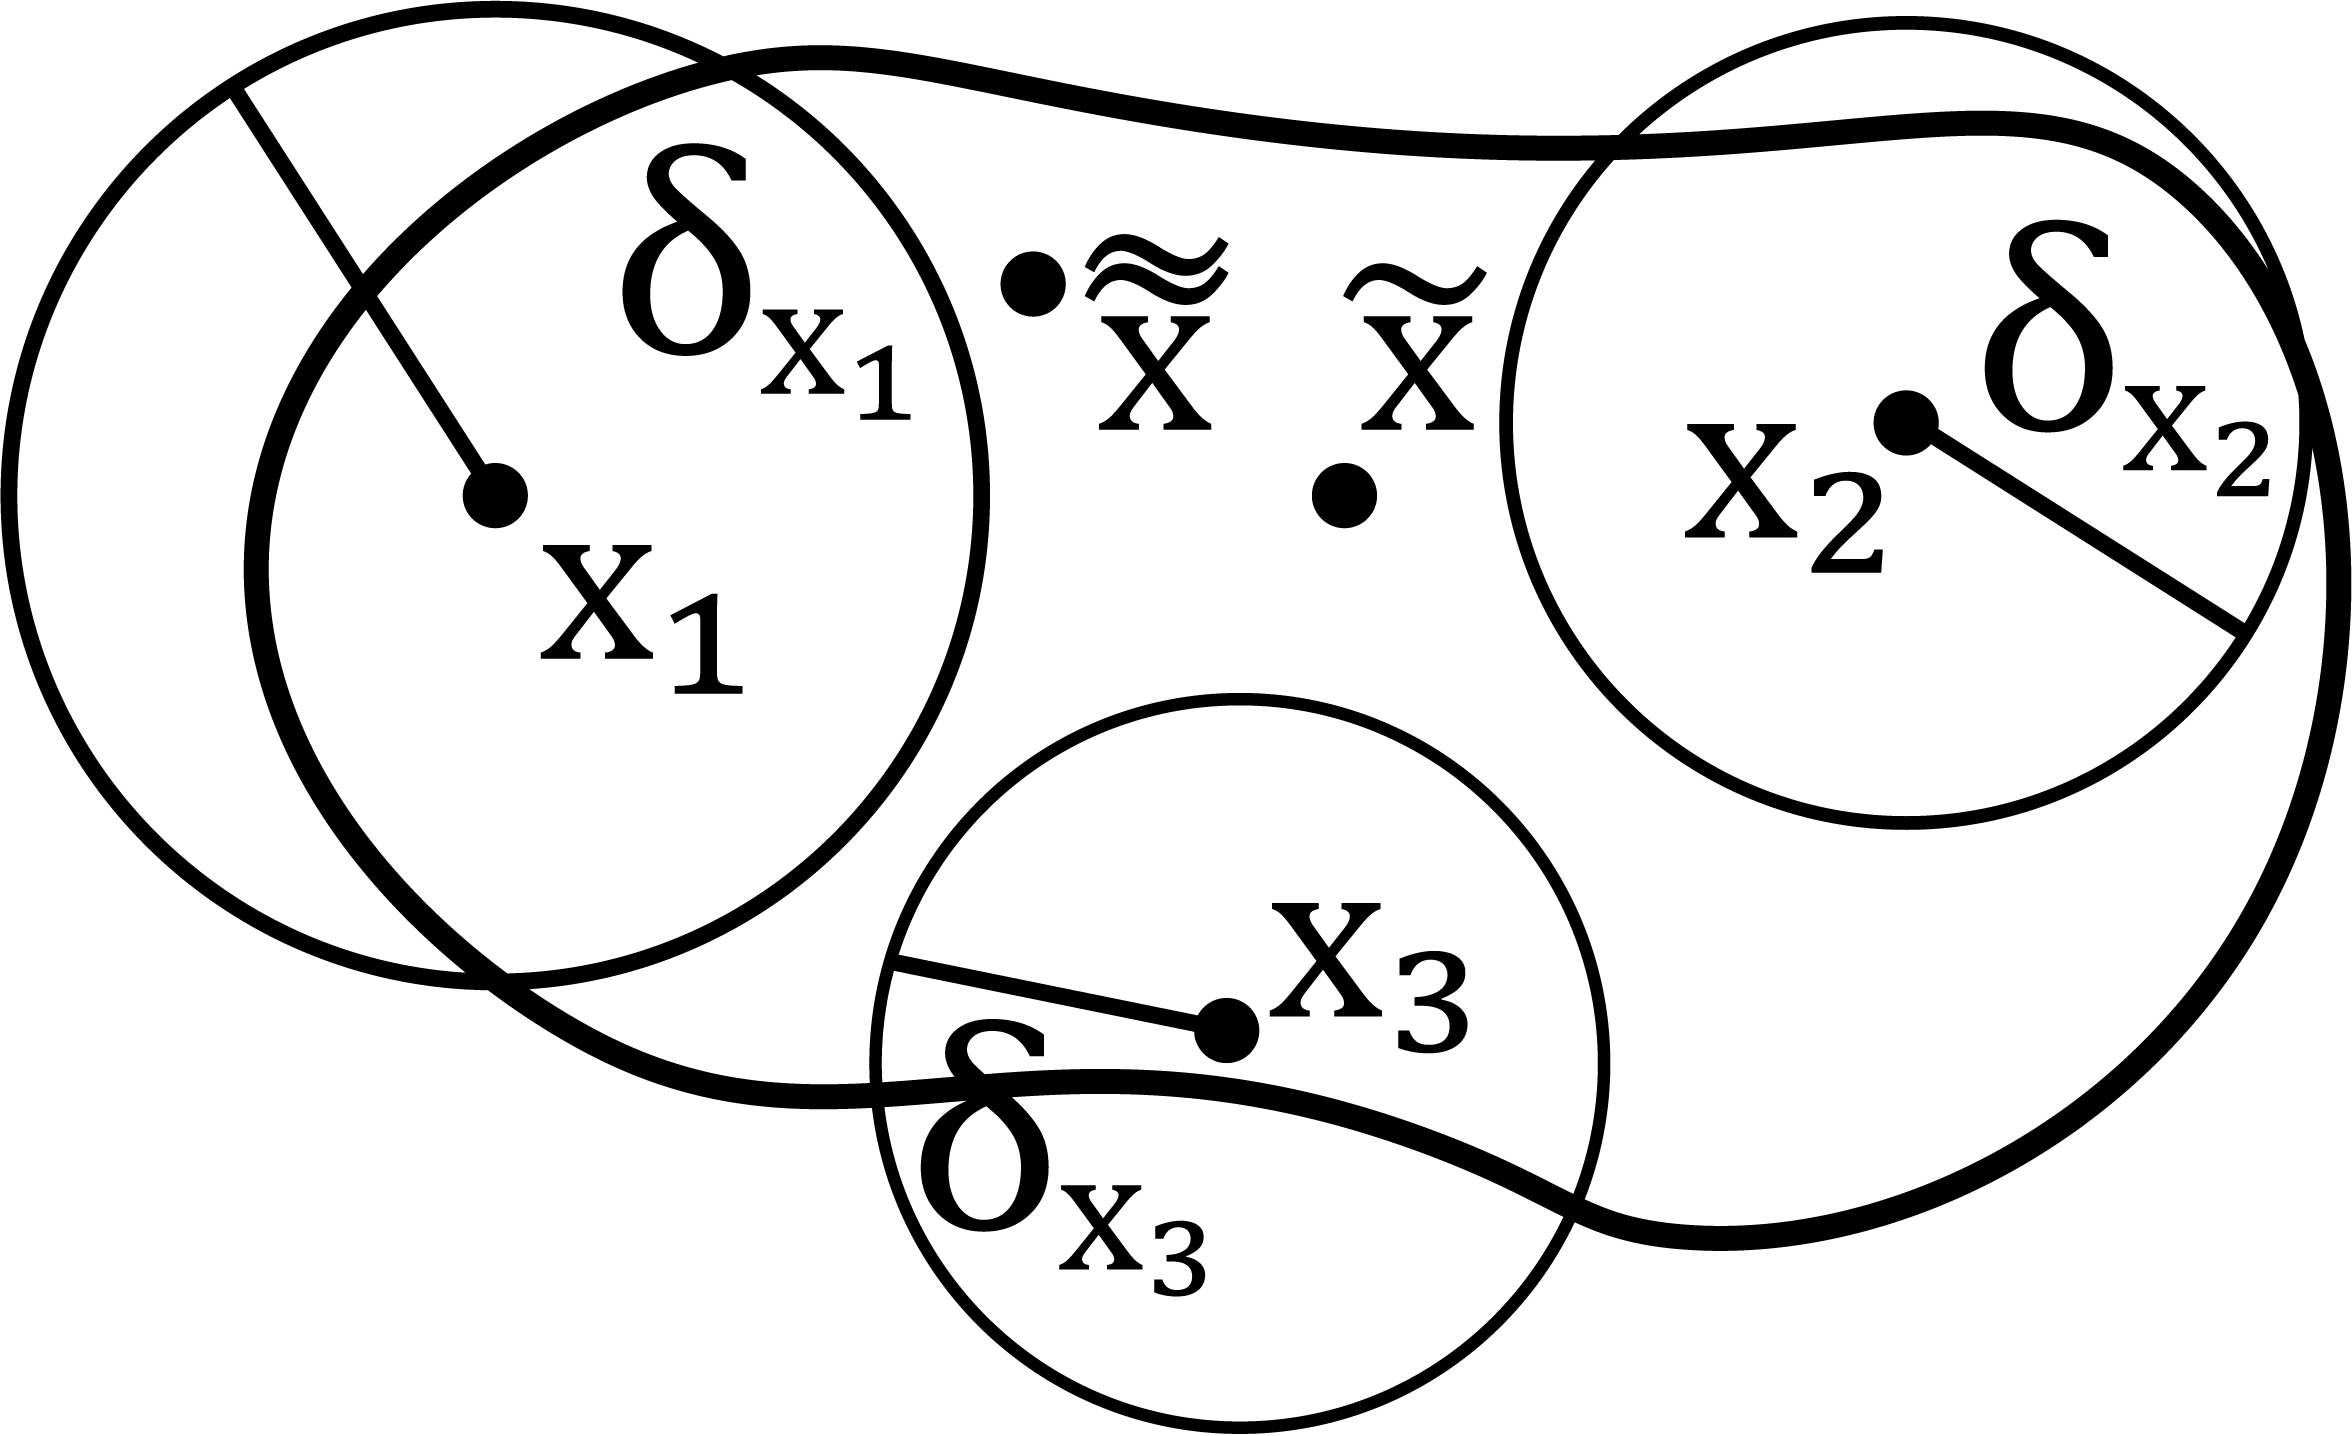
\includegraphics[width = 5cm]{pics/3_3}}
		\[\{B_x(\delta_x)\}_{x \in K} \text{ --- откр. покрытие комп. }K \]
		\[\text{Выделим конечное поддпокрытие}\]
		\[K \subset \bigcup_{j = 1}^N B_{x_j} (\delta_{x_j} )\]
		\[\delta = \min_{1 \leq j \leq N} \delta_{x_j} \text{ --- то, что надо} \]
		\[\text{Пусть } d(\widetilde{x}, \widetilde{\widetilde{x}}) < \delta\]
		\[\widetilde{x} \in K \RA \exists x_l : \widetilde{x} \in B(x_l, \delta_{x_l}) \]
		\[d(\widetilde{\widetilde{x}}, x_l) \leq d(\widetilde{\widetilde{x}}, \widetilde{x}) +
			d(\widetilde{x}, x_l) < \delta + \delta_{x_l}  < 2 \delta_{x_l} \]
		\[\Ra d(f(\widetilde{\widetilde{x}}), f(x_l)) < \frac{\mathcal{E}}{2}\q\text{и} \q d(f(\widetilde{x}), f(x_l)) < \frac{\mathcal{E}}{2}\]
		\[d(f(\widetilde{x}), f(\widetilde{\widetilde{x}})) \leq
			d(f(\widetilde{x}), f(x_l)) + d(f(\widetilde{\widetilde{x}}), f(x_l)) < \mathcal{E}\]
	\end{Proof}

	\newpage
	\subsection{Линейные  операторы  в $\R^n$.  Норма  линейного  оператора,  корректность определения}

	\begin{Definition}
		\[\text{Норма в } \R^n: \q ||\cdot||: \R^n \to [0, +\infty)\]
		Аксиомы нормы
		\begin{enumerate}
			\item $||x|| \geq 0$
			\item $||x|| = 0 \rla x = 0$
			\item $||k \cdot x|| = |k| \cdot ||x||$
			\item $||x + y|| \leq ||x|| + ||y||$
		\end{enumerate}
		Стандартная норма в $\R^n$:
		\[||x|| = d(x, 0) = \sqrt{\sum_{k = 1}^n |x_k|^2 }\]
		Проверим аксиому 4:
		\[||x+y|| = d(x+y, 0) = d(x, -y) \leq d(x, 0) + d(0, -y) = ||x|| + ||y||\]
	\end{Definition}

	\begin{upr}[1]
		Пусть $||| \cdot |||$ --- другая норма в $\R^n$\\
		Тогда \q$\exists c, C > 0:$
		\[c \cdot ||x|| \leq |||x||| \leq C \cdot ||x|| \q \forall x \in \R^n\]
	\end{upr}

	\begin{upr}[2]
		$\forall$ норма непр. в $\R^n$
	\end{upr}

	\begin{Definition}
		\[x, y \in \R^n \qq x \cdot y = (x,\ y) = \sum_{j = 1}^n x_j y_j \]
		\[||x||^2 = (x,\ x)\]
		Н-во К-Б: $(x, y)^2 \leq ||x||^2 \cdot ||y||^2$
	\end{Definition}

	\begin{Definition}
		\[\LL(\R^n, \R^m) \text{ --- лин. операторы}\]
		\[L \in \LL (\R^n, \R^m): \forall x, y \in \R^n; \q \forall a, b \in \R:\]
		\[L(ax + by) = aL(x) + bL(y)\]
		Пишут $Lx \text{ вместо } L(x)$
		\[\LL(\R^n, \R^m) \text{ --- лин. пр-во:}\]
		\[\text{Если } A, B \in \LL(\R^n, \R^m), \text{ то } (A + B) (x) = Ax + Bx\]
		\[A + B \in \LL(\R^n, \R^m)\]
		\[\forall k \in \R\q (kA)(x):= k \cdot Ax\]
		\[kA \text{ --- тоже лин. оператор}\]
		Кроме того $A \in \LL(\R^n, \R^m),\q B \in \LL(\R^k, \R^n)$
		\[AB = A \circ B \in \LL(\R^k, \R^m)\]
		Пусть $\{e_j\}_{j = 1}^n $ --- базис (ортонорм) в $\R^n$; \q $\{e^*_j\}_{j = 1}^m $ - базис в $\R^m$
		\[\text{Тогда } \forall \text{ лин. оператору соотв. }Mat(A)\]
		\[Ae_j = \sum_{k=1}^m a_{k_j} e^*_k  \q\q Mat(A) = \begin{pmatrix}
				a_{11} & a_{1j} & ... & a_{1n} \\
				...                            \\
				a_{m1} & a_{mj} & ... & a_{mn}
			\end{pmatrix}\]
		\[\LL(\R^n, \R^m) \simeq Mat_\R (m \times n) \simeq \R^{mn} \]
		\[Mat(A \circ B) = Mat(A) \cdot Mat(B) \text{ --- матричное произв.}\]
		\[A \in \LL(\R^n, \R^m) \q B \in \LL(\R^k, \R^n)\]
	\end{Definition}

	\begin{Theorem}
		\[\LL(\R^n, \R^m) \subset C(\R^n, \R^m)\]
	\end{Theorem}

	\begin{Proof}
		\[d(x, y) = ||x - y||\]
		\[A : \R^n \to  \R^m \text{ --- лин. оператор}\]
		\[||Ax - Ay|| = ||\underset{A( \os{n}{\us{j = 1}{\sum}} (x_j - y_j) e_j )}{A(x-y)}|| =
			|| \sum^{n}_{j = 1}  (x_j - y_j) \cdot Ae_j|| \leq\]
		\[\leq \sum^{n}_{j = 1} |x_j - y_j| \cdot ||Ae_j|| \leq M \sqrt{n} ||x - y||\]
		\[M = \max_{1 \leq j \leq n} ||Ae_j|| \q\q \forall \mathcal{E} > 0 \q \exists
			\delta = \frac{\mathcal{E}}{M \sqrt{n}}\]
	\end{Proof}

	\[B_0(1) = \{x \in \R^n : ||x|| \leq 1\} \text{ --- компакт}\]
	\[A \in \LL(\R^n, \R^m) \text{ --- непр. на } B_0(1) \RA \text{ огр.}\]
	\[||Ax|| \text{ --- непр. } \R^n \to  \R\]
	\[\Ra \text{ достигает наиб. знач. на комп. } B_0(1)\]

	\begin{Consequence}
		\[\sup_{||x|| \leq 1}  ||Ax|| = \max_{||x|| \leq 1} ||A x|| < \infty \]
	\end{Consequence}

	\newpage
	\subsection{Теорема о равносильных определениях нормы линейного оператора}

	\begin{Definition}
		\[A \in \LL(\R^n, \R^m)\]
		\[\text{Норма лин. оператора } A\]
		\[||A|| = \max_{|x| \leq 1} ||A x|| \]
	\end{Definition}

	\begin{Theorem}
		\[||A|| = \max_{||x|| = 1}  ||Ax|| = \sup_{||x|| \neq 0}  \frac{||A x||}{||x||}\]
		\[\text{т.е. } \forall x \in \R^n \q ||A x|| \leq ||A|| \cdot ||x||\]
	\end{Theorem}

	\begin{Proof}
		\[\text{Если } A \equiv 0 \text{ --- очев.} \q (||A|| = 0)\]
		\[\text{Пусть } A \not \equiv 0 \RA \exists x^* \in \R^n \setminus \{0\} : ||Ax^*|| \neq 0\]
		\[0 \neq \frac{||Ax^*||}{||x^*||} = \Abs{A \frac{x^*}{\underset{= y^* \in s_1 \subset B_0}{||x^*||}}} \RA ||A|| > 0\]
		Пусть max достигается внутри ед. шара:
		\[||A|| = ||A \widetilde{x}||, \text{ где } ||\widetilde{x}|| < 1\]
		\[\text{Рассм. } \widetilde{y} = \frac{\widetilde{x}}{||x||}\]
		\[||A\widetilde{y}|| = \frac{||A\widetilde{x}||}{||\widetilde{x}||} > ||A\widetilde{x}||, \text{ т.е. } ||A\widetilde{x}|| \text{ не max!}\]
		\[\Ra \max ||Ax|| \text{ в } ||x|| \leq 1 \q \text{ достиг. на сфере } ||x|| = 1\]
		\[||A|| = \max_{||x|| = 1} ||A_x|| \]
		\[||A|| = \max_{||x|| = 1} ||Ax|| = \sup_{||x|| = 1} \frac{||Ax||}{||x||} \leq
			\sup_{||x|| \neq 0} \frac{||Ax||}{||x||} \]
		\[\sup_{||x|| \neq 0} \frac{||Ax||}{||x||} = \sup_{||x|| \neq 0} ||A \frac{x}{||x||}|| \leq
			\max_{||y|| = 1} ||Ay|| = ||A|| \]
	\end{Proof}

	\newpage
	\subsection{Теорема  о  том,  что  норма  линейного  оператора  ---  действительно норма}

	\begin{theorem}
		\begin{enumerate}
			\item Норма оператора, действительно, норма
			\item $||A \cdot B|| \leq ||A|| \cdot ||B||$
		\end{enumerate}
	\end{theorem}

	\begin{proof}
		\begin{enumerate}
			\item Проверим аксиомы нормы:
			      \[(1)\q ||A|| \geq 0 \text{ --- очев.}\]
			      \[(2)\q ||A|| = 0 \rla A = 0 \text{ (начало предыдущей теоремы)}\]
			      \[(3)\q ||k \cdot A|| = \max_{||x|| = 1} ||(k \cdot A)x|| =
				      \max_{||x|| = 1} |k| \cdot ||Ax|| = |k| \cdot ||A|| \]
			      \[(4)\q ||A + B|| = \max_{||x|| = 1} ||Ax + Bx|| \leq \max_{||x|| = 1} (||Ax|| + ||Bx||) \leq \]
			      \[\leq ||A|| + ||B||\]
			\item $\displaystyle ||(AB)x|| = ||A(Bx)|| \leq ||A|| \cdot ||Bx|| \leq
				      ||A|| \cdot ||B|| \cdot ||x||$
			      \[\sup_{||x|| \neq 0} \frac{||ABx||}{||x||} \leq ||A|| \cdot ||B||\]
			      \[\sup = ||AB||\]
		\end{enumerate}
	\end{proof}

	\newpage
	\subsection{Оценка нормы линейного оператора}

	\begin{Theorem}[оценка нормы лин. оператора]
		\[A \in \LL (\R^n, \R^m) \q Mat(A) = \begin{pmatrix}
				a_{11} & ... & a_{1n} \\
				...                   \\
				a_{m1} & ... & a_{mn}
			\end{pmatrix}\]
		\[||A||^2 \leq \sum^m_{i = 1} \sum^n_{j = 1} |a_{ij}|^2  = ||A||^2_{HS} \text{ --- норма Гильберта Шмидта} \]
	\end{Theorem}

	\begin{Proof}
		\[y = Ax = A(\sum_{j = 1}^n \cdot x_j \cdot e_j) = \sum^n_{j = 1} x_j \cdot Ae_j \]
		\[\underset{\text{k-я координата }}{y_k} = \sum^n_{j = 1}x_j(Ae_j)_k \text{ --- к-я координата} \]
		\[1 \leq k \leq m\]
		\[|y_k|^2 = |\sum^n_{j = 1} x_j (Ae_j)_k|^2 \leq \sum_{j = 1}^n |x_j|^2 \cdot
			\sum^n_{j=1} \underset{= a_{jk} }{(Ae_j)_k^2} = ||x||^2 \sum^n_{j = 1} |a_{kj}| \]
		\[y = \begin{pmatrix}
				y_1    \\
				y_2    \\
				\vdots \\
				y_m
			\end{pmatrix}
			= \begin{pmatrix}
				a_{11} & a_{12} & ... & a_{1n} \\
				a_{21} & a_{22} & ... & a_{2n} \\
				...                            \\
				a_{m1} & ...    & ... & a_{mn}
			\end{pmatrix}
			\begin{pmatrix}
				x_1    \\
				x_2    \\
				\vdots \\
				x_n
			\end{pmatrix}
		\]
		\[||y||^2 = ||Ax||^2 = \sum^m_{k = 1}|y_k|^2 \leq ||x||^2 \cdot \sum^m_{k = 1}\sum^n_{j = 1} |a_{kj}|^2\]
		\[||A|| = \sup_{||x|| \neq 0} \frac{||Ax||}{||x||} \leq \sqrt{\sum^m_{k = 1} \sum^n_{j = 1} |a_{kj}| }\]
	\end{Proof}

	\begin{Upr}
		\[||A||_{HS} \leq \sqrt{n} \cdot ||A||\]
	\end{Upr}

	\newpage
	\subsection{Дифференцируемость отображения, дифференциал. Примеры}

	\begin{Definition}
		\[E \subset \R^n, \q E \text{ --- откр.} \q a \in E\]
		\[f: E \to  \R^m\]
		\[f \text{ --- дифф-мо в т. } a \text{, если } \exists L \in \LL(\R^n, \R^m)\]
		\[f(a + h) = f(a) + Lh + \underset{\alpha(h)}{o(||h||)} \q\q ||h|| \to  0\]
		\center{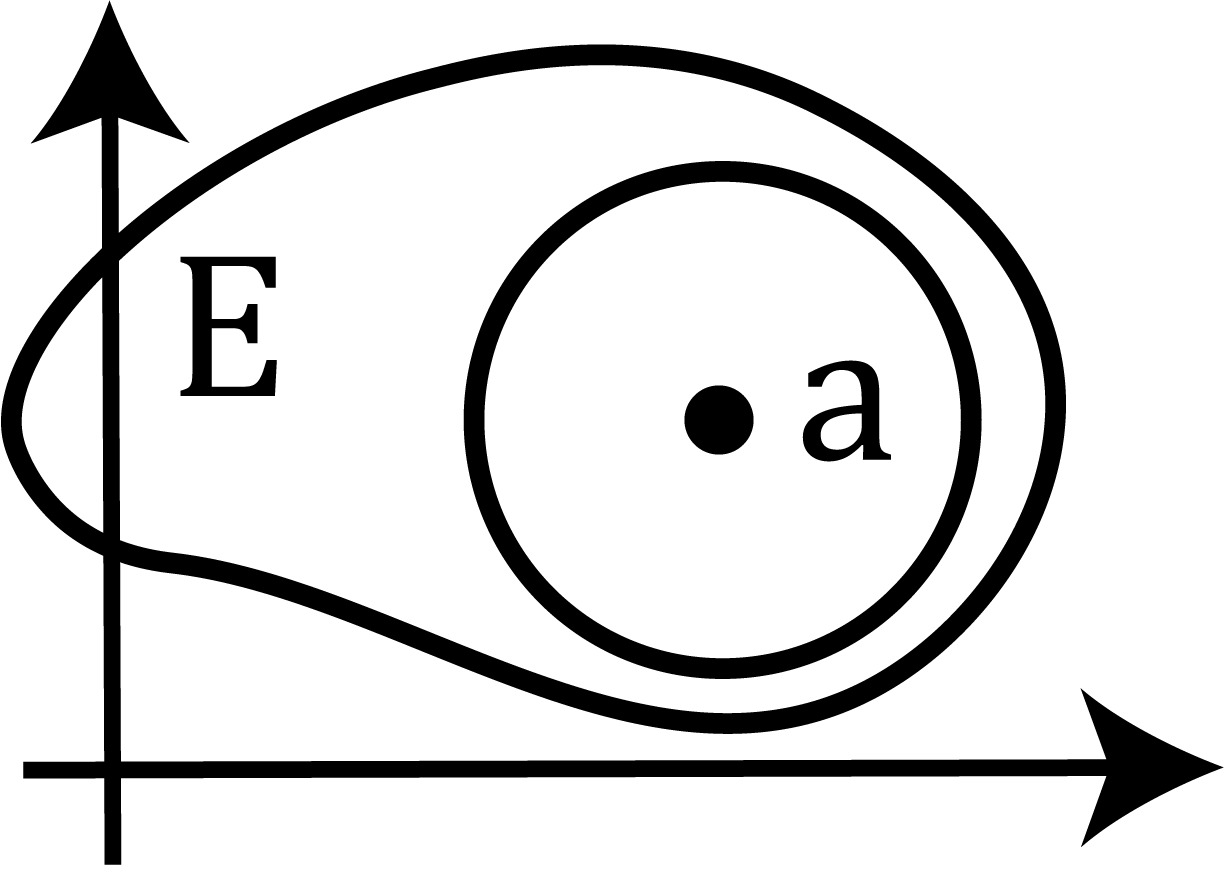
\includegraphics[width = 2.5cm]{pics/3_4}}
		\[(h: a + h \in E)\]
		\[\alpha(h) = o(||h||) = o(h) \rla \lim_{||h|| \to 0} \frac{||\alpha(h)||}{||h||} = 0 \]
		\[f(a + h) = f(a) + Lh + o(||h||) \rla \lim_{||h|| \to 0} \frac{||f(a+h) - f(a) - Lh||}{||h||} = 0\]
		Если такой L $\exists$, то он ед.
		\[\text{Пусть } h \in \R^n : ||h|| = 1\]
		\[a + t \cdot h\]
		\center{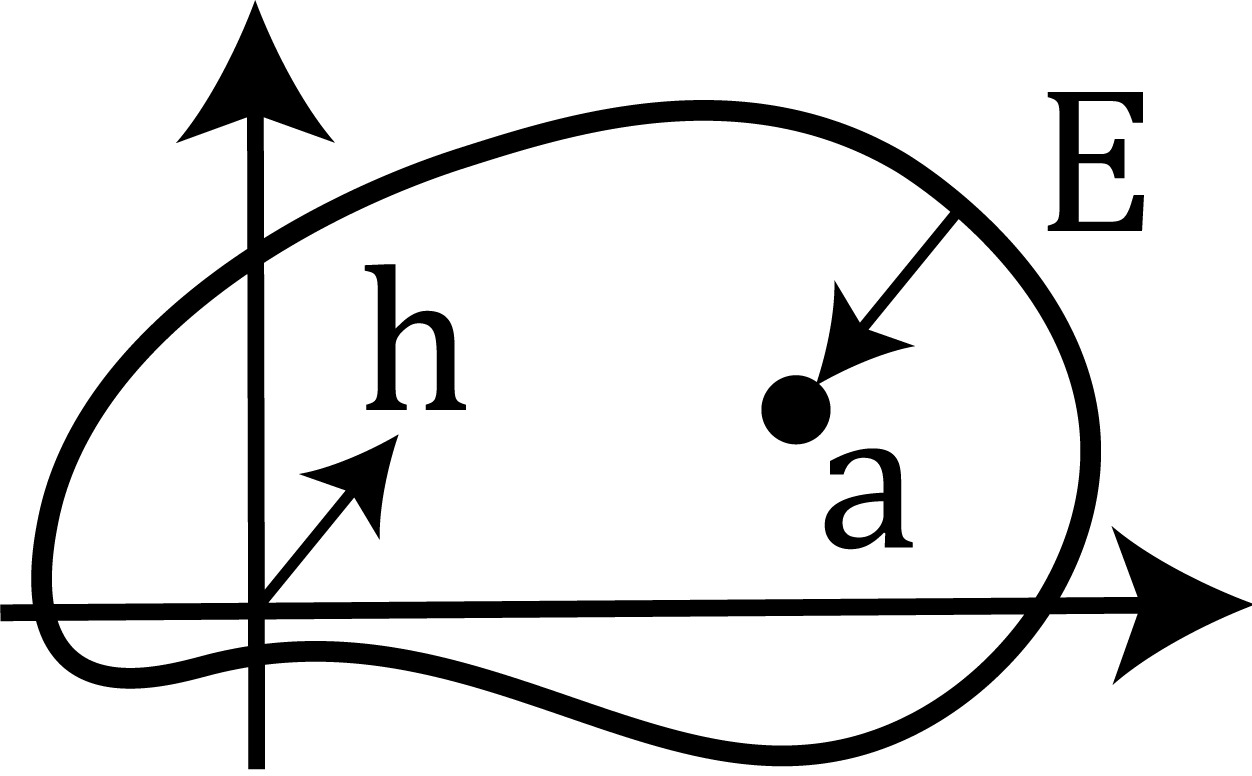
\includegraphics[width = 3cm]{pics/3_5}}
		\[f(a + th) = f(a) + \underbrace{L(th)}_{= t \cdot Lh}  + o(th)\]
		\[||th|| \to  0\]
		\[\frac{f(a + th)f(a)}{t} = Lh + \frac{o(th)}{t} \underset{t \to 0}{\to 0}\]
		\[Lh = \lim_{t \to  0} \frac{f(a + th) - f(a)}{t} \]
		\[\forall h : ||h|| = 1 \q L \text{ опеределен однозначно } \ra \forall x \neq 0\]
		\[Lx = ||x|| \cdot L \frac{x}{||x||}\]
		\[L \text{ --- дифференциал. } f \text{ в т. а}\]
		\[d_a f = L \in \LL(\R^n, \R^m)\]
		\[h \in \R^n \q\q d_a f(h) \in \R^m\]
	\end{Definition}

	\begin{Examples}
		\[\lim_{||h|| \to  0} \frac{||f(a + h) - f(a) - Lh||}{||h||} = 0\]
		\begin{enumerate}
			\item $f = \const \RA d_a f = 0$
			\item $f \in \LL(\R^n, \R^m) = f(a + h) - f(a) = f(h) \RA Lh = f(h)$
			      \[d_a f = f \text{ (если f --- линейна)}\]
			\item Если $f, g : \R^n \to \R^m $ - диф. в т. a, то
			      \[d_a(f + g) = d_a f + d_a g\]
			      \[\lim_{||h|| \to 0}  \frac{||(f + g)(a + h) - (f + g)(a) - d_a f(h) - d_a g(h)||}{||h||} = \]
			      \[ \leq \lim_{} \frac{|| f(a + h) - f(a) - d_a f(h)|| + || g(a + h) - g(a) - d_a g(h)||}
				      {||h||}  = 0\]
			\item $d_a(kf) = kd_a f$
		\end{enumerate}
	\end{Examples}

	\newpage
	\subsection{Производная по направлению, связь с дифференциалом. Частные
производные}

	\begin{Definition}
		\[\text{Пусть } ||e|| = 1, \q e \in \R^n \q\q f:E \to \R^m \q a \in E\]
		\[\frac{\partial f}{\partial e}(a) = \lim_{t \to 0} \frac{f(a + te) - f(a)}{t} \]
	\end{Definition}

	\begin{Theorem} [о производной по напр.]
		\[f : E \to \R^m \text{ --- дифф. в т. } a\]
		\[\frac{\partial f}{\partial e} (a) = d_a f(e)\]
		\center{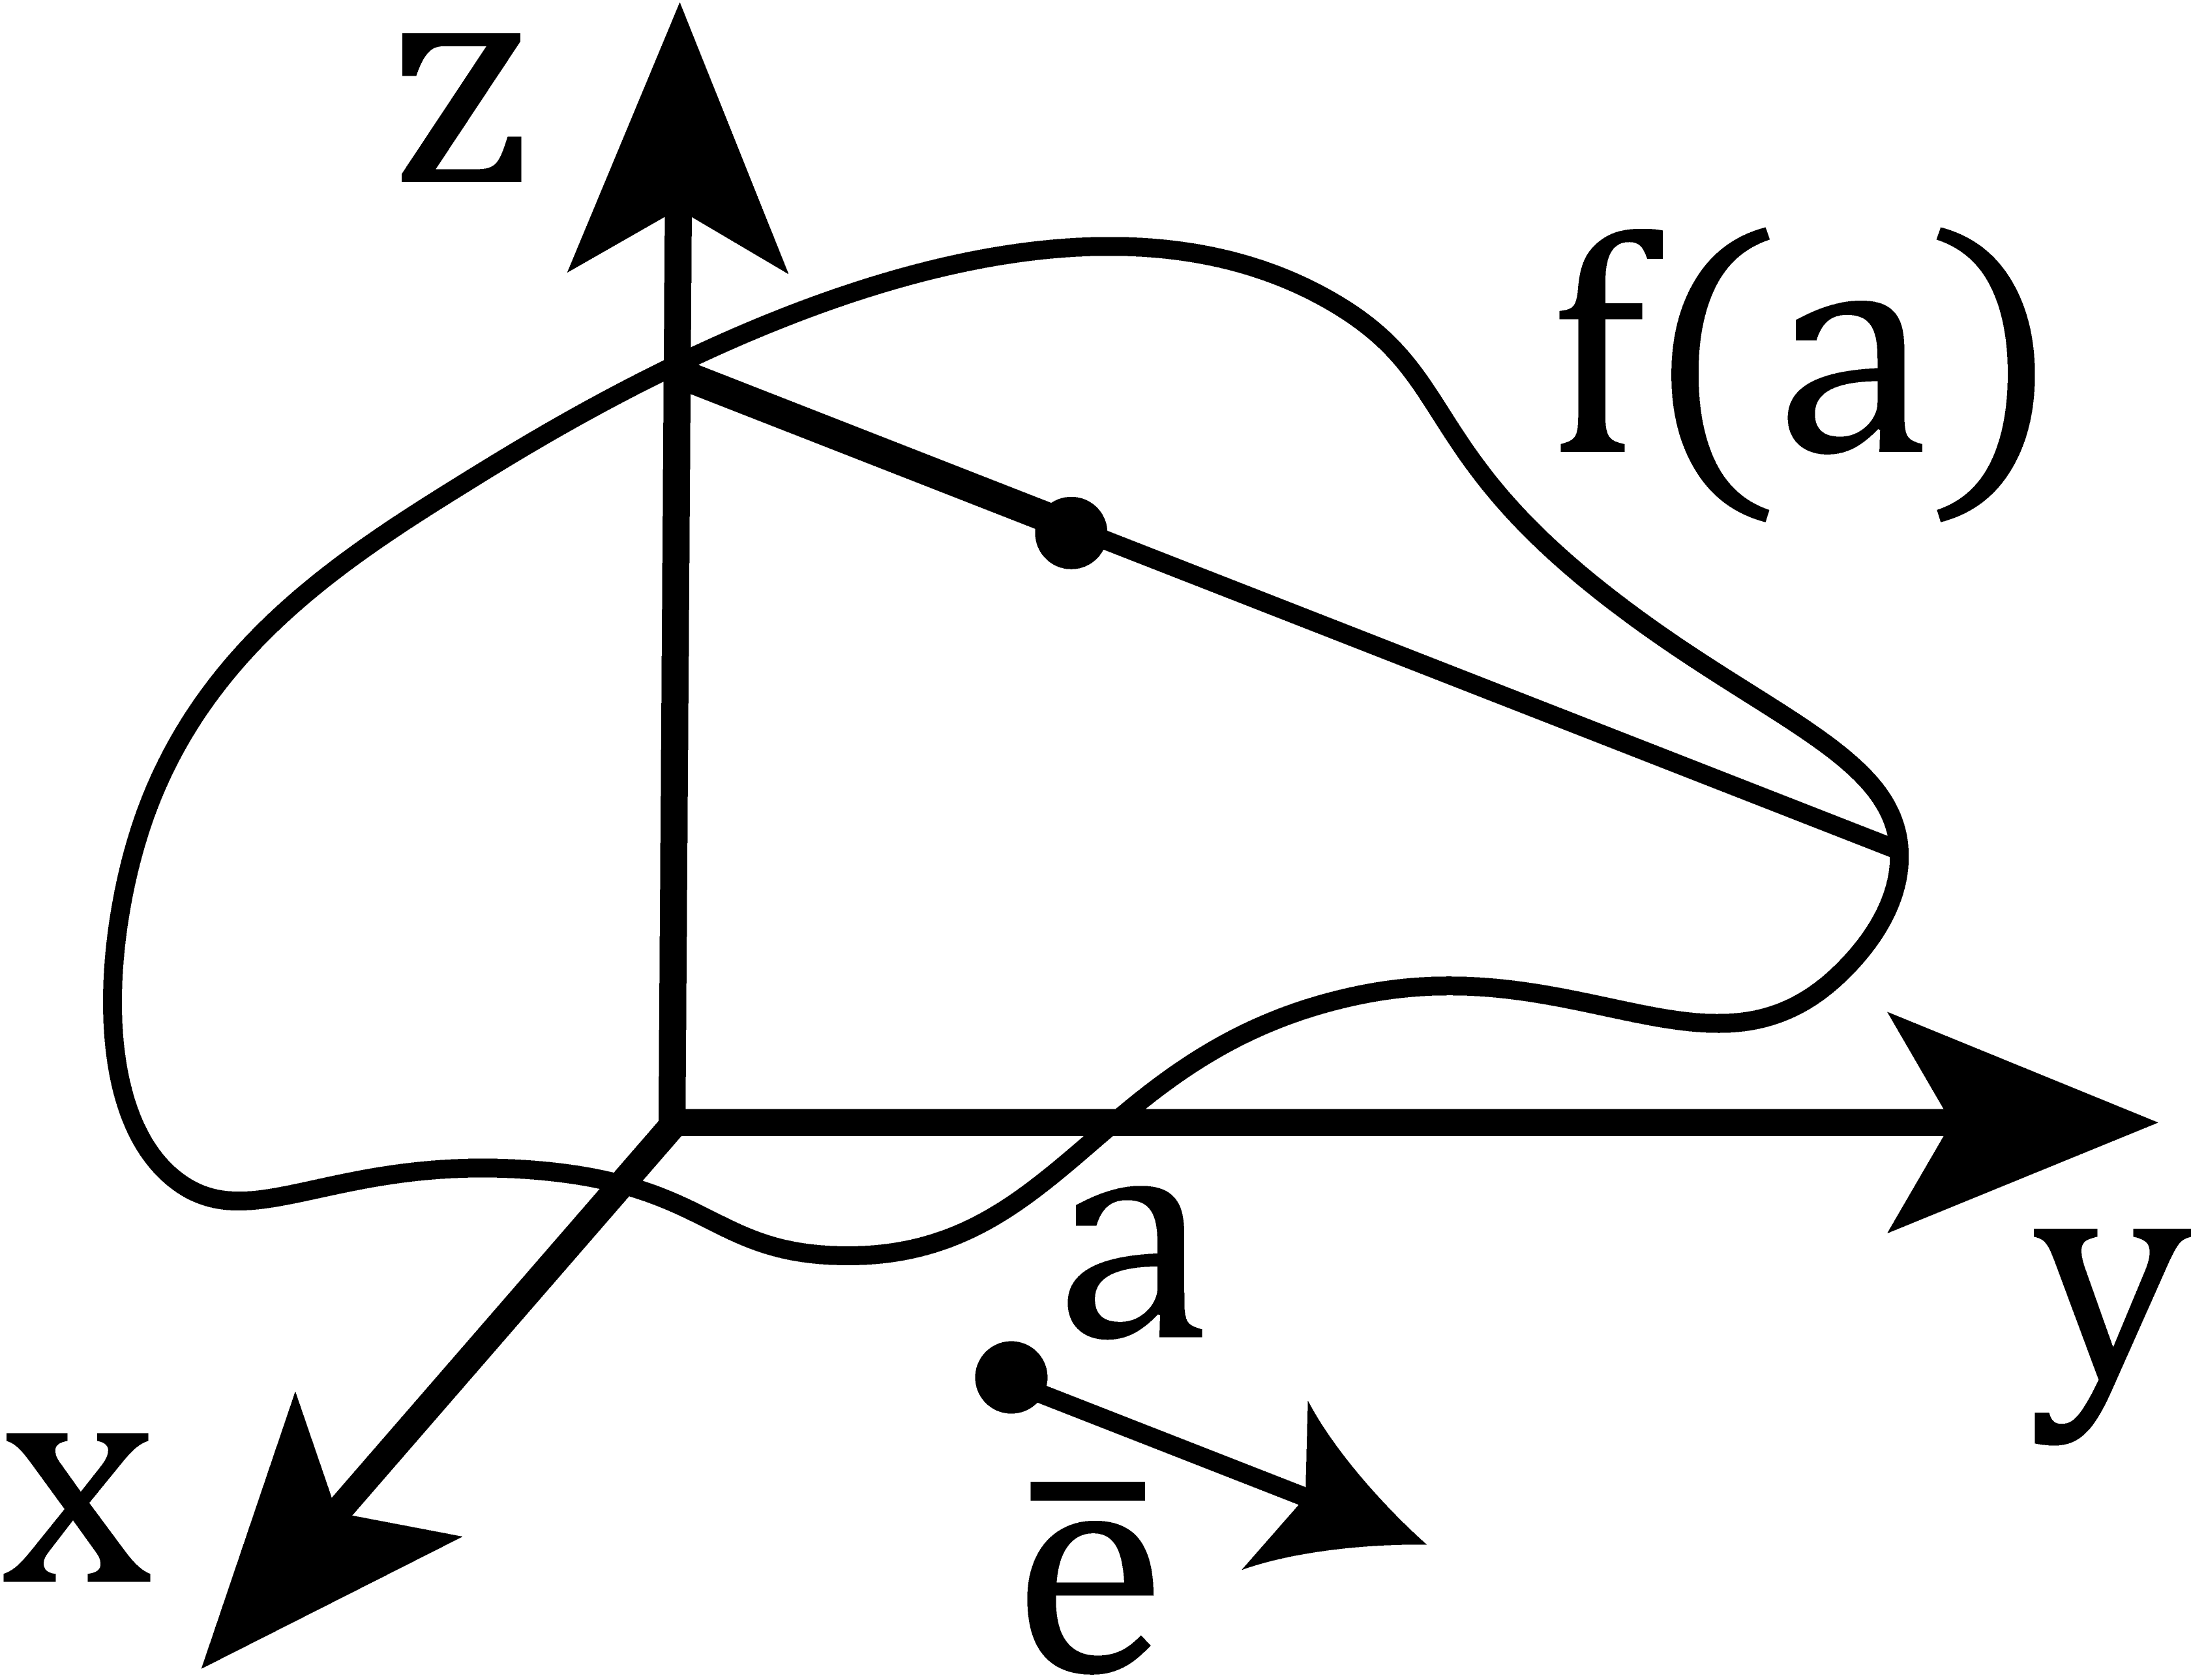
\includegraphics[width = 3cm]{pics/3_6}}
		\[z = f(x, y)\]
		\[f: E \to \R^1 \q\q E \subset \R^2\]
	\end{Theorem}

	\begin{Proof}
		\[f(a + te) - f(a) - d_a f(te) + o(te) \q ||te|| \to 0 \q\q ||te|| = |t|\]
		\[\frac{\partial f}{\partial e}(a) = \lim_{t \to 0} \frac{f(a + te) - f(a)}{t} = d_a f(e)\]
	\end{Proof}

	\begin{definition}
		Частные производные $\{e_k\}_{k = 1}^n $ --- базис $\R^n$
		\[f : E \to \R^m \q\q E \subset \R^n \q a \in E\]
		\[\frac{\partial f}{\partial x_k}(a) = f_{x_k}' (a) = \frac{\partial f}{\partial e_k}(a)\]
	\end{definition}

	\newpage
	\subsection{Теорема о дифференцировании композиции}

	\begin{Definition}
		\[\text{Пусть } f \text{ --- диф. в т. } a \in E\]
		\[\text{Временно вернемся к обозначению} \q L = d_a f\]
		\[Mat(L) \text{ --- матрица Якоби}\]
		\[\begin{pmatrix}
				a_{11} & a_{12} & ... & a_{1n} \\
				\vdots &        &     & \vdots \\
				a_{m1} & a_{m2} & ... & a_{mn}
			\end{pmatrix} \q \text{$j$-й столбец --- координаты вектора } \]
		\[d_a f (e_j) = \frac{\partial f}{\partial e_j}(a) = \frac{\partial f}{\partial x_j}(a) \q\q 1 \leq j \leq n\]
		\[a_{kj}  = \frac{\partial f_k}{\partial x_j}(a)\]

		\[\Mat(d_af) = \begin{pmatrix}
				\frac{\partial f_1}{\partial x_1}(a) & ...    & \frac{\partial f_1}{\partial x_n} (a) \\
				\vdots                               & \ddots & \vdots                                \\
				\frac{\partial f_m}{\partial x_1}(a) & ...    & \frac{\partial f_m}{\partial x_n} (a)
			\end{pmatrix}\]
	\end{Definition}
\end{document}
